% !TEX program = xelatex
\documentclass[11pt]{article}

% ---------- gói (biên dịch bằng XeLaTeX cho tiếng Việt) ----------
\usepackage{fontspec}
% Nạp Latin Modern theo tên tệp OTF (có sẵn trong TeX Live/Overleaf và tectonic);
% hỗ trợ đầy đủ dấu tiếng Việt. Biên dịch bằng XeLaTeX.
\setmainfont{lmroman10-regular.otf}[
  BoldFont=lmroman10-bold.otf,
  ItalicFont=lmroman10-italic.otf,
  BoldItalicFont=lmroman10-bolditalic.otf]
\setmonofont{lmmono10-regular.otf}
\usepackage[margin=1in]{geometry}
\usepackage{microtype}
\usepackage{graphicx}
\usepackage{booktabs}
\usepackage{amsmath}
\usepackage{amssymb}
\usepackage{array}
\usepackage{multirow}
\usepackage{caption}
\usepackage{xcolor}
\usepackage{listings}
\usepackage{enumitem}
\usepackage{placeins}
\usepackage[hidelinks]{hyperref}

\graphicspath{{figures/}}

% ---------- bản địa hoá tiếng Việt cho tên các đối tượng ----------
\renewcommand{\contentsname}{Mục lục}
\renewcommand{\abstractname}{Tóm tắt}
\renewcommand{\refname}{Tài liệu tham khảo}
\renewcommand{\tablename}{Bảng}
\renewcommand{\figurename}{Hình}
\renewcommand{\appendixname}{Phụ lục}

% ---------- kiểu hiển thị prompt / mã nguồn ----------
\definecolor{promptbg}{gray}{0.96}
\lstdefinestyle{prompt}{
  basicstyle=\ttfamily\footnotesize,
  backgroundcolor=\color{promptbg},
  frame=single,
  framesep=6pt,
  breaklines=true,
  columns=fullflexible,
  keepspaces=true,
  xleftmargin=4pt,
  xrightmargin=4pt,
}
\lstset{style=prompt}

\newcommand{\todo}[1]{\textcolor{red}{\textbf{[CẦN LÀM: #1]}}}

% ---------- tiêu đề ----------
\title{\textbf{Hệ thống LLM đa tác tử y khoa nhằm nâng cao độ chính xác thực tế trên MedQA-USMLE}\\[4pt]
\large Báo cáo giữa kỳ}
\author{Nguyễn Đình Thanh \and Ngô Văn Tú \and Lê Viết Hưng \and Trần Quốc Phong}
\date{}
\emergencystretch=3em

\begin{document}

% ---------- trang bìa ----------
\begin{titlepage}
\thispagestyle{empty}
\begin{center}
{\large ĐẠI HỌC QUỐC GIA TP. HỒ CHÍ MINH}\\
{\bfseries\large TRƯỜNG ĐẠI HỌC CÔNG NGHỆ THÔNG TIN}\\[2pt]
\rule{0.55\textwidth}{0.6pt}\\[24pt]

\IfFileExists{figures/uit_logo.pdf}{%
  
\includegraphics[height=3cm]{uit_logo.pdf}\\[22pt]%
}{%
  \fbox{\parbox[c][3cm][c]{3cm}{\centering\textcolor{red}{\bfseries [LOGO UIT]}}}\\[22pt]%
}

{\large MÔN HỌC: MÁY HỌC TRONG BẢO MẬT MẠNG VÀ HỆ THỐNG}\\[50pt]

{\Large\bfseries HỆ THỐNG LLM ĐA TÁC TỬ Y KHOA NHẰM NÂNG CAO}\\[4pt]
{\Large\bfseries ĐỘ CHÍNH XÁC THỰC TẾ TRÊN MEDQA-USMLE}\\[12pt]
{\large Báo cáo giữa kỳ}\\[50pt]

\begin{minipage}{0.75\textwidth}
\textbf{Giảng viên hướng dẫn:} Lê Kim Hùng\\[8pt]
\textbf{Nhóm thực hiện:} Nhóm 01\\[8pt]
\textbf{Thành viên:}
\begin{itemize}[nosep, leftmargin=2.4cm]
  \item Nguyễn Đình Thanh - 250202053
  \item Ngô Văn Tú - 250202057
  \item Lê Viết Hưng - 250202040
  \item Trần Quốc Phong - 250202051
\end{itemize}
\end{minipage}

\vfill
TP. Hồ Chí Minh, 2026
\end{center}
\end{titlepage}

% ---------- mục lục, trang riêng ----------
\newpage
\thispagestyle{empty}
\tableofcontents
\newpage

\begin{abstract}
Nhóm xây dựng và đánh giá một hệ thống LLM đa tác tử (multi-agent) y khoa dạng module với mục
tiêu nâng cao \emph{độ chính xác thực tế} (factual accuracy) trên bộ dữ liệu MedQA-USMLE. Hệ thống được
tổ chức thành một \textbf{thang biến thể} (ablation ladder) gồm năm biến thể (V0 LLM trực
tiếp $\rightarrow$ V4 hệ đa tác tử đầy đủ); mỗi biến thể chỉ là cùng một sơ đồ xử lý (StateGraph) của
LangGraph, nhưng bật/tắt vài thành phần theo một cấu hình định sẵn tương ứng. Nhờ hai biến thể liền
nhau chỉ khác đúng một thành phần, mọi chênh lệch về độ chính xác đều quy thẳng được về thành phần đó. Tất cả biến thể dùng chung một giao diện thống nhất và một bộ đo (độ chính xác kèm khoảng tin cậy
bootstrap, tỷ lệ phản hồi không hợp lệ, phân tích Thắng/Thua/Hòa, và kiểm định ghép cặp McNemar), giúp
phép so sánh trung thực. Phát hiện thực nghiệm cốt lõi của Nhóm là: trên MedQA \textbf{riêng truy
hồi (retrieval) không giúp ích} (V1: $-1.7$ điểm so với V0, không có ý nghĩa thống kê), trong khi
\textbf{lập luận đa tác tử mới là bước cải thiện thực sự đầu tiên} (V2: $+5.3$ điểm, McNemar
$p{=}0.044$) - đo trên 300 câu đầu của tập test; bộ kiểm chứng (V3) hiện chưa cho thấy cải thiện thêm
so với V2 ở quy mô này. Nhóm trình bày kết quả đo hiện tại, ghi lại đầy đủ kiến trúc, prompt và cấu
hình truy hồi để tái lập được, đồng thời liệt kê các phần việc còn lại để đạt tới đánh giá chính thức
đầy đủ trên toàn bộ 1273 câu.
\end{abstract}
\bigskip

% =====================================================================
\section{Giới thiệu}
% =====================================================================
Các mô hình ngôn ngữ lớn (LLM) trả lời đúng nhiều câu hỏi thi y khoa ngay từ đầu, nhưng cũng đưa ra
những câu trả lời sai một cách rất tự tin, và không dễ thấy \emph{thành phần kiến trúc nào} thực sự làm
giảm những lỗi đó. MedAgents~\cite{tang2024medagents} cung cấp bằng chứng ban đầu rằng phối hợp đa tác tử
theo dạng hội đồng chuyên gia - các tác tử độc lập đề xuất phân tích, sau đó đi đến đồng thuận - cải
thiện lập luận y khoa zero-shot trên MedQA-USMLE; nhưng hệ thống đó gộp đồng thời nhiều thành phần (truy
hồi, hội đồng, nhiều vòng thảo luận), khiến khó tách biệt đóng góp riêng của từng yếu tố. Nghiên cứu này đặt
câu hỏi thiết kế: \emph{bắt đầu từ một LLM thuần, mỗi thành phần - truy hồi tri thức (RAG), phối hợp
đa tác tử (multi-agent), và bước kiểm chứng (verifier) - đóng góp bao nhiêu vào độ chính xác thực tế
trên MedQA-USMLE?}

\paragraph{Bài toán.} Đầu vào là một câu hỏi trắc nghiệm MedQA-USMLE~\cite{jin2021medqa} (một tình huống lâm sàng kèm bốn
lựa chọn A-D). Đầu ra bắt buộc là \emph{đúng một} lựa chọn cuối cùng cộng với một giải thích ngắn
($\le 30$ từ).

\paragraph{Cách tiếp cận.} Nhóm không thực hiện tách rời năm hệ thống riêng biệt. Thay vào đó, mỗi biến thể
là \emph{cùng một} bộ khung LangGraph~\cite{langgraph2024}, chỉ bật/tắt các nút (node) khác nhau theo
một cấu hình định sẵn, và mỗi bậc chỉ bổ sung \emph{đúng một} thành phần so với bậc trước: V0$\to$V1
thêm truy hồi agentic (RAG), V1$\to$V2 tách một tác tử duy nhất thành bốn nút chuyên trách - hiểu ca
bệnh, tìm kiếm, lập luận, quyết định (Mục~\ref{sec:variants}) - V2$\to$V3 thêm bộ kiểm chứng và bộ
nhớ ngắn hạn, còn V3$\leftrightarrow$V4 bật/tắt đúng bộ kiểm chứng đó. Thiết kế bốn nút này khác hẳn
hội đồng nhiều chuyên gia kiểu MedAgents mà Nhóm đã thử trước khi ổn định trên kiến trúc hiện tại
(\S\ref{sec:variants}). Vì một bộ đo duy nhất chấm cả năm biến thể theo cùng một bộ đánh giá, mọi
chênh lệch điểm số đều so sánh được trực tiếp.

\paragraph{Đóng góp của nhóm nghiên cứu.}
\begin{enumerate}[nosep]
  \item Một kiến trúc đa tác tử điều khiển bằng cấu hình (V0-V5) - việc khám phá ban đầu lấy cảm
  hứng từ MedAgents~\cite{tang2024medagents}, nhưng kiến trúc hiện tại là một thiết kế bốn nút riêng
  của Nhóm (Mục~\ref{sec:variants}) - trong đó mỗi cải tiến khác phiên bản trước đó đúng một thành
  phần (Mục~\ref{sec:arch}-\ref{sec:design}).
  \item Một quy trình đánh giá ghép cặp, tái lập được, có kiểm định ý nghĩa thống kê
  (Mục~\ref{sec:setup}-\ref{sec:results}).
  \item Kết quả thực nghiệm cho thấy trên MedQA, \emph{cấu trúc lập luận đa tác tử}, chứ không phải
  \emph{truy hồi}, mới là yếu tố làm thay đổi độ chính xác - nhất quán với lý giải của MedAgents
  nhưng lần đầu được tách biệt qua thiết kế ablation có kiểm soát
  (Mục~\ref{sec:results}-\ref{sec:discussion}).
\end{enumerate}

\paragraph{Trạng thái đo lường.} Kiến trúc (V0-V4) đã được xây dựng đầy đủ và kiểm tra chạy được
đầu-cuối. Báo cáo này đo V0-V3 trên kiến trúc \emph{hiện tại} (thiết kế bốn nút + luật tin cậy bất
đối xứng, \S\ref{sec:design}) ở $n{=}300$/1273 câu test (\S\ref{sec:results}): V2 là cải thiện có ý
nghĩa thống kê đầu tiên so với V0 ($p{=}0.044$); V1 (retrieval) và V3 (+ bộ kiểm chứng) chưa cho thấy
khác biệt có ý nghĩa so với V0. V4 chưa được đo. Mỗi khoảng trống còn lại (đo ở $n{=}1273$, đo V4) đều
được đánh dấu \todo{} để người đọc biết chính xác điều gì đã đo và điều gì mới là dự kiến.

% =====================================================================
\FloatBarrier
\section{Kiến trúc hệ thống}
\label{sec:arch}
% =====================================================================
Ý tưởng là tạo một bộ khung ứng dụng duy nhất với các nút được bật/tắt tuỳ biến thể:
\[
\text{understand}\;\rightarrow\;(\text{search}\parallel\text{reasoning})\;\rightarrow\;\text{decide}\;\rightarrow\;\text{[verify]}\;\rightarrow\;\text{[distill\_mistake]}
\]
Một biến thể không được tạo bởi một nhánh mã riêng, mà nó phụ thuộc vào một \texttt{RunConfig} định sẵn, sau đó được biên dịch thành
một \texttt{StateGraph} của LangGraph~\cite{langgraph2024} qua \texttt{build\_graph(cfg)}.

\begin{figure}[tbp]
  \centering
  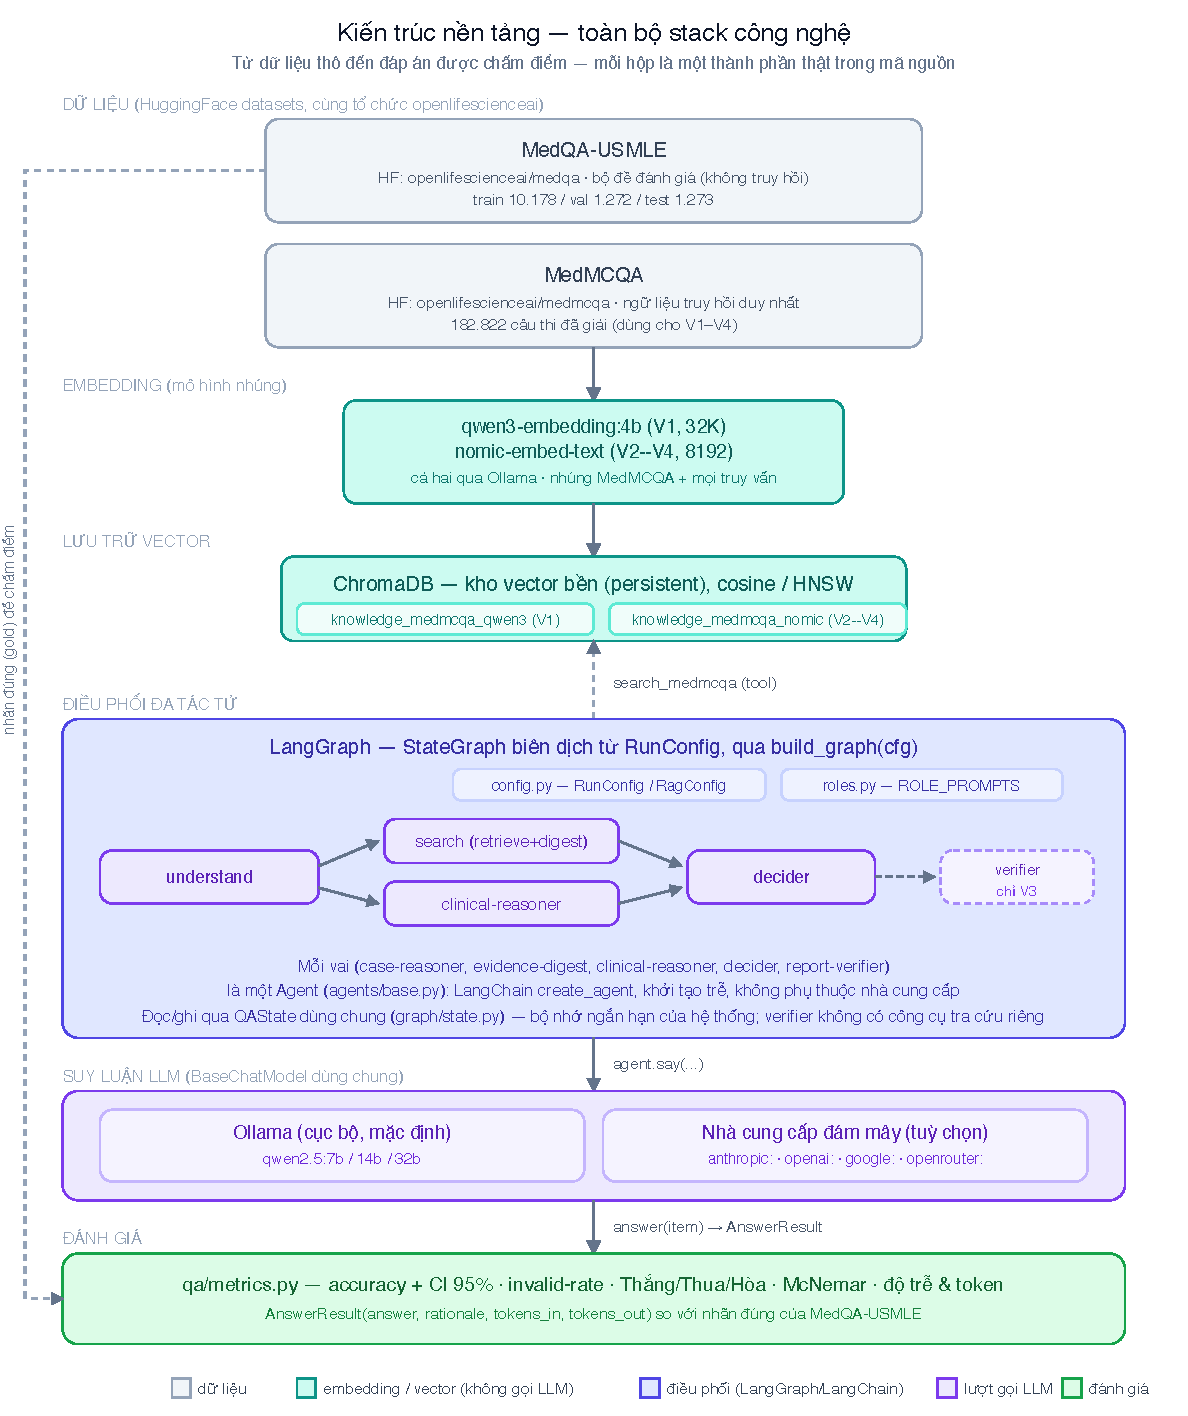
\includegraphics[width=\textwidth,height=0.82\textheight,keepaspectratio]{system_stack.pdf}
  \caption{Technology stack: từ dữ liệu thô đến đáp án được chấm.}
  \label{fig:stack}
\end{figure}

\paragraph{Vai trò từng thành phần trong stack (Hình~\ref{fig:stack}).}
\begin{itemize}[nosep]
  \item \textbf{Dữ liệu (HuggingFace \texttt{datasets}):} \textbf{MedQA-USMLE}~\cite{jin2021medqa} là bộ
  đề dùng để đánh giá, không bao giờ dùng để truy hồi; \textbf{MedMCQA}~\cite{pal2022medmcqa} là dữ
  liệu truy hồi duy nhất, dùng chung cho toàn bộ V1-V5.
  \item \textbf{Embedding:} một embedder duy nhất qua Ollama cho toàn bộ V1-V5 - \textbf{qwen3-embedding:4b}
  (ngữ cảnh 32K token). V2-V5 dùng một embedder ngữ cảnh ngắn hơn (8192 token) ở một thiết kế trước đó,
  nhưng đã chuyển sang cùng embedder với V1 sau một A/B nhỏ - xem \S\ref{sec:rag}.
  \item \textbf{Lưu trữ vector - ChromaDB:} vector persistent database, đo độ tương đồng bằng Cosine Estimation, một
  bộ sưu tập duy nhất (\texttt{knowledge\_medmcqa\_qwen3}), dùng chung cho V1-V5.
  \item \textbf{Bộ nhớ dài hạn (cross-episode) - SqliteStore:} persistent database cho nhiều round
  (\texttt{data/longterm/}, \texttt{graph/longterm.py}), tách biệt với \texttt{QAState} (bộ nhớ ngắn
  hạn trong một câu). Hai namespace độc lập: \texttt{medqa-lessons} - bài học chung mà \texttt{decider}
  tự recall/remember (từ V3), và \texttt{medqa-mistakes} - kho tiến hoá các ca đã trả lời SAI mà
  \texttt{verify} recall và \texttt{distill\_mistake} remember (chỉ V5, \S\ref{sec:memory}).
  \item \textbf{Điều phối đa tác tử - LangGraph:} \texttt{StateGraph} biên dịch một \texttt{RunConfig}
  (\texttt{config.py}) thành đồ thị các nút (\texttt{graph/nodes.py}, \texttt{graph/build.py}); mọi nút
  đọc/ghi qua \texttt{QAState} dùng chung (\texttt{graph/state.py}) - đây chính là kênh giao tiếp chính của
  các nodes trong hệ thống (\S\ref{sec:memory}).
  \item \textbf{Tác tử - LangChain:} mỗi role trong đồ thị (tối đa 6 roles ở V5, xem Hình~\ref{fig:stack})
  là một \texttt{Agent} (\texttt{agents/base.py}), bọc \texttt{create\_agent} của LangChain - khởi tạo
  không phụ thuộc nhà cung cấp mô hình LLM. Prompt của từng role nằm trong \texttt{roles.py}.
  \item \textbf{Suy luận LLM:} \textbf{Ollama} cục bộ (\texttt{qwen2.5:7b}) là mặc định;
  các nhà cung cấp đám mây (\texttt{anthropic:}, \texttt{openai:}, \texttt{google:},
  \texttt{openrouter:}) gọi bằng interface \texttt{BaseChatModel} qua tham số
  \texttt{provider:model} (\S\ref{sec:setup}).
  \item \textbf{Đánh giá:} \texttt{qa/metrics.py} so \texttt{AnswerResult} (đáp án, giải thích, token)
  với nhãn đúng của MedQA-USMLE, tính độ chính xác kèm khoảng tin cậy bootstrap, tỷ lệ không hợp lệ,
  Thắng/Thua/Hòa, và McNemar (\S\ref{sec:results}).
\end{itemize}

\begin{figure}[tbp]
  \centering
  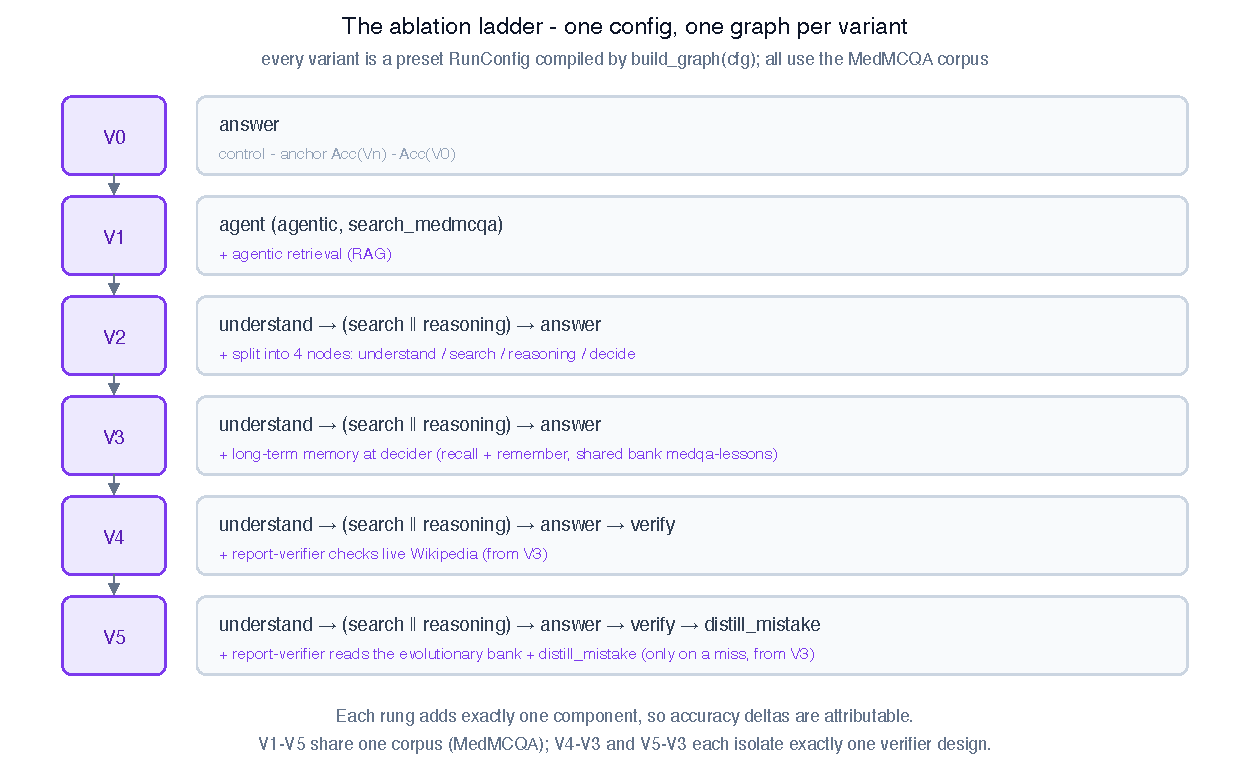
\includegraphics[width=0.95\textwidth]{ladder_overview.pdf}
  \caption{Thang ablation: mỗi biến thể thêm đúng một khả năng.}
  \label{fig:ladder}
\end{figure}

\begin{table}[h]
  \centering
  \caption{Các nút thực sự được nối trong mỗi biến thể (tên nút khớp với mã nguồn).}
  \label{tab:variants}
  \small
  \begin{tabular}{@{} c l c @{}}
    \toprule
    Biến thể & Các nút tác tử  & Số lượng tác tử \\
    \midrule
    V0 & \texttt{answer} & 1 \\[3pt]
    V1 & \texttt{agent}\; (agentic, gọi \texttt{search\_medmcqa}) & 1 \\[3pt]
    V2 & \texttt{understand\;$\rightarrow$\;(search\;$\|$\;reasoning)\;$\rightarrow$\;answer} & 4 \\[3pt]
    V3 & \texttt{understand\;$\rightarrow$\;(search\;$\|$\;reasoning)\;$\rightarrow$\;answer}\;+\;long-term memory & 4 \\[3pt]
    V4 & V3's graph\;+\;\texttt{verify}\;(Wikipedia-grounded) & 5 \\[3pt]
    V5 & V3's graph\;+\;\texttt{verify}\;+\;\texttt{distill\_mistake} & 6 \\
    \bottomrule
  \end{tabular}
\end{table}

V1 là ngoại lệ của bộ khung trên: thay vì tách \texttt{understand}/\texttt{search}/\texttt{reasoning}
thành các nút riêng, nó rút về một nút \texttt{agent} duy nhất, tự làm cả bốn việc trong một lượt hội
thoại có gọi công cụ (xem \S\ref{sec:rag}). V2-V5 theo đúng bộ khung bốn nút, với Node~1
(\texttt{understand}) sinh ra bản tóm tắt ca bệnh + truy vấn dùng chung cho hai nhánh Node~2
(\texttt{search}) và Node~3 (\texttt{reasoning}) chạy \emph{đồng thời}, trước khi Node~4
(\texttt{answer}, vai \texttt{decider}) tổng hợp; V3 không thêm nút nào (\texttt{decider} tự đọc/ghi
bộ nhớ dài hạn), V4/V5 mỗi biến thể thêm các nút sau \texttt{answer} (Node~5 thêm 
\texttt{verify}; V5 thêm cả Node~6 \texttt{verify} và \texttt{distill\_mistake}).

\FloatBarrier
% =====================================================================
\section{Thiết kế hệ thống}
\label{sec:design}
% =====================================================================

\subsection{Các biến thể: V0-V5}
\label{sec:variants}
Mỗi tác tử là một lớp khởi tạo quanh \texttt{create\_agent} của LangChain với một
\texttt{BaseChatModel} không phụ thuộc nhà cung cấp. Mục này giới thiệu từng biến thể theo đúng thứ tự thang
ablation - luồng xử lý, các tác tử tham gia, và điều mỗi layer thêm vào so với layer trước; \S\ref{sec:rag}
đi sâu hơn vào các quyết định thiết kế dùng chung cho V1-V5.

\paragraph{V0 - LLM trực tiếp (baseline).} Một LLM duy nhất, không RAG: \texttt{format\_mcq} dựng prompt (tình huống + A-D), model trả lời, \texttt{parse\_choice}
trích chữ cái. Đây là mốc mà mọi biến thể khác được so sánh vào: \text{Độ chính xác}(Vn) $-$
\text{Độ chính xác}(V0).

\begin{figure}[tbp]
  \centering
  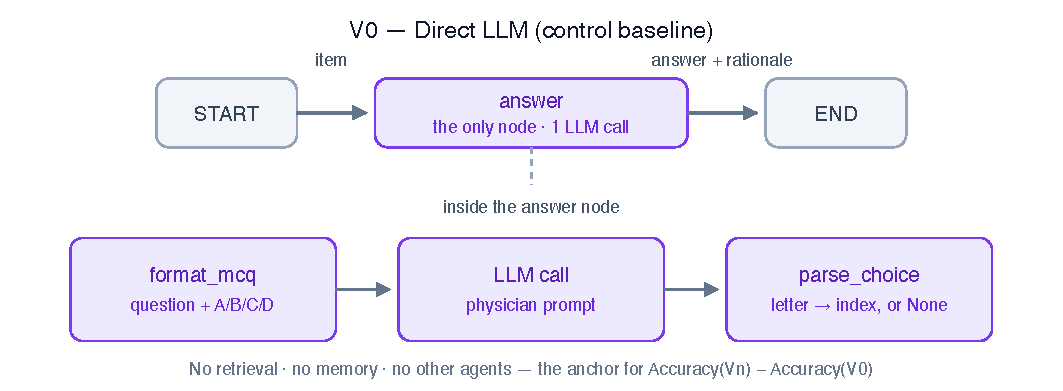
\includegraphics[width=0.92\textwidth]{v0_flow.pdf}
  \caption{V0: một node, không RAG.}
  \label{fig:v0}
\end{figure}

\paragraph{V1 - một tác tử agentic RAG.} Đồ thị rút về một node: \texttt{START $\rightarrow$ agent
$\rightarrow$ END}. Bên trong, \texttt{Agent(rag-agent)} tự quyết định có gọi \texttt{search\_medmcqa}
hay không (tối đa hai lần), tự chấm độ tin cậy của bằng chứng lấy về (HIGH/MEDIUM/LOW), rồi áp luật
\emph{tin cậy bất đối xứng} (\S\ref{sec:rag}) để chốt đáp án - tất cả trong cùng một tác tử, không
có node/tác tử riêng cho từng bước.

\begin{figure}[tbp]
  \centering
  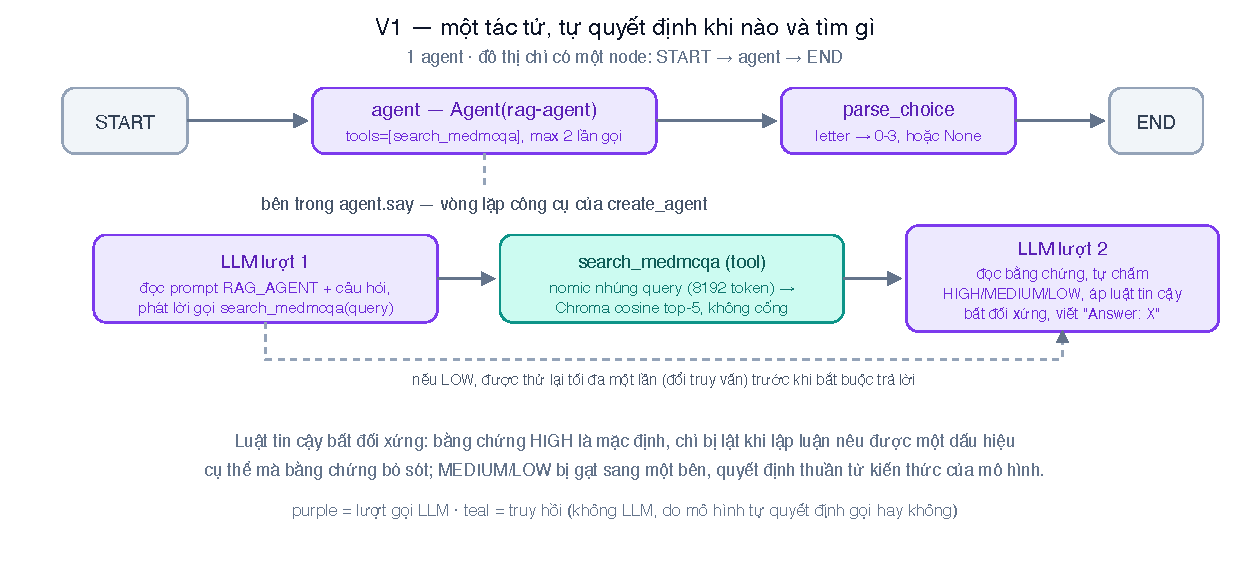
\includegraphics[width=\textwidth]{v1_flow.pdf}
  \caption{V1: một tác tử agentic tự gọi công cụ và tự quyết định.}
  \label{fig:v1}
\end{figure}

\paragraph{V2 - bốn nút: hiểu ca bệnh, tìm kiếm, lập luận, quyết định.} V2-V4 dùng chung một thiết
kế bốn nút, được tách dựa trên bốn việc mà tác tử đơn của V1 làm bên trong nó,
được tạo và kết nối thông qua LangGraph:
\begin{itemize}[nosep]
  \item \textbf{Node~1 - \texttt{case-reasoner} (\texttt{hiểu ca bệnh}):} đọc tình huống một lần, viết
  ra một bản tóm tắt ca bệnh và một truy vấn tìm kiếm, dùng cho hai nút sau.
  \item \textbf{Node~2 - \texttt{search} (tìm kiếm + rút gọn):} gọi \texttt{search\_medmcqa} với
  truy vấn của Node~1, rồi \texttt{evidence-digest} tóm bằng chứng thành một đoạn ngắn kèm mức tin cậy
  tự đánh giá.
  \item \textbf{Node~3 - \texttt{clinical-reasoner} (\texttt{lập luận}):} lập luận từ bản tóm
  tắt của Node~1, hoàn toàn không thấy bằng chứng của Node~2 (hai nhánh chạy đồng thời); tự chấm mức
  tin cậy của chính lập luận đó.
  \item \textbf{Node~4 - \texttt{decider} (\texttt{quyết định}):} nhận hai đầu vào độc lập kèm mức tin
  cậy riêng, áp luật tin cậy bất đối xứng để chốt đáp án.
\end{itemize}

\begin{figure}[tbp]
  \centering
  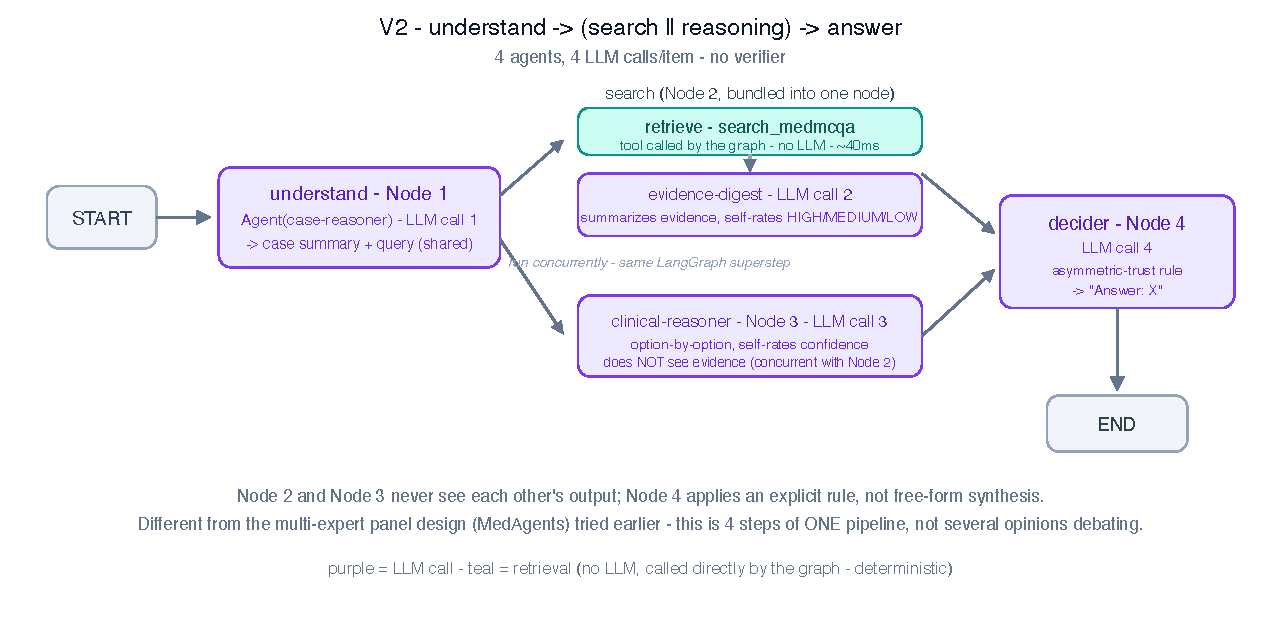
\includegraphics[width=\textwidth]{v2_flow.pdf}
  \caption{V2: Node 1 phân nhánh song song sang Node 2/3, hội tụ ở Node 4.}
  \label{fig:v2}
\end{figure}

\paragraph{V3 - V2 nhưng \texttt{decider} có bộ nhớ dài hạn.} V3 giữ nguyên bốn nút của V2, nhưng bật
\texttt{long\_term=True}: Node~4 (\texttt{decider}) tự \texttt{recall} bài học từ các câu TƯƠNG TỰ đã
gặp trước đó trước khi chốt đáp án, rồi tự
\texttt{remember} lại một bài học sau khi chốt - không cần một tác tử riêng cho việc
"nhớ", thông qua tool \texttt{remember/recall} mà \texttt{decider} sẵn có.

\begin{figure}[tbp]
  \centering
  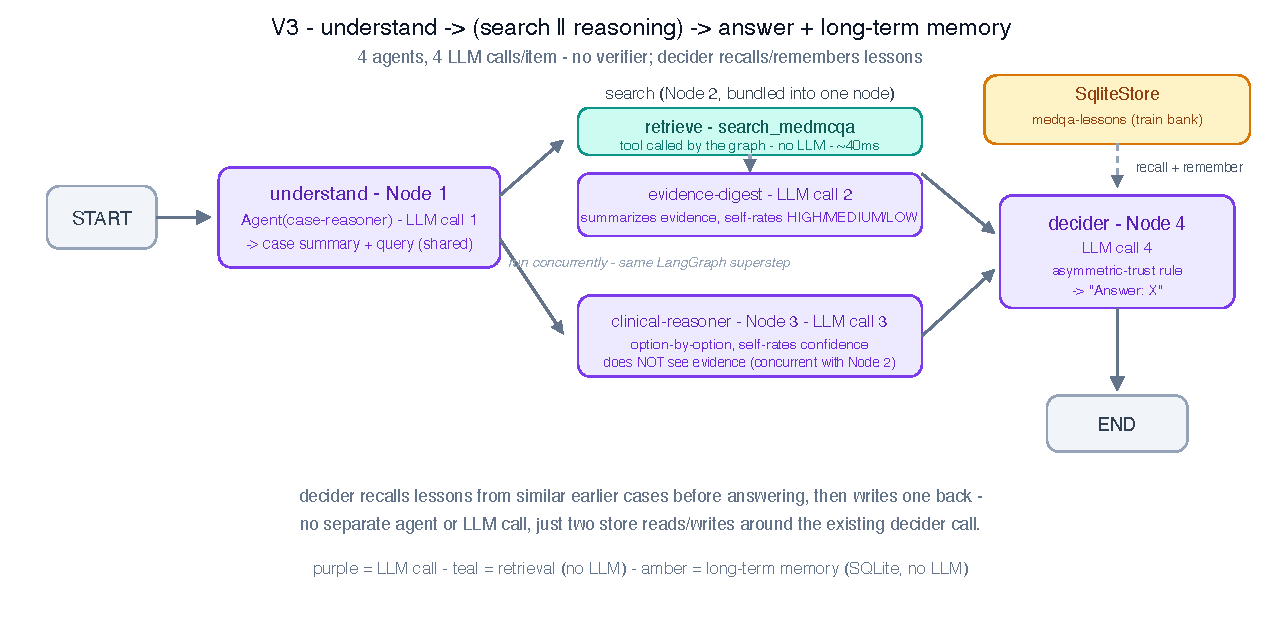
\includegraphics[width=\textwidth]{v3_flow.pdf}
  \caption{V3: bốn nút của V2; \texttt{decider} tự \texttt{recall}/\texttt{remember} vào
  \texttt{medqa-lessons}.}
  \label{fig:v3}
\end{figure}

\paragraph{V4 - V3 + bộ kiểm chứng đối chiếu Wikipedia.} V4 thêm \textbf{Node~5 -
\texttt{report-verifier}}: đọc lại báo cáo lập luận của Node~3 và bản tóm tắt ca bệnh của Node~1
(\texttt{memory=True}), rồi xác nhận hoặc chỉnh đáp án của
Node~4 (\S\ref{sec:verifier}). Khi báo cáo không đủ để quyết, nó gọi tool \texttt{search\_wikipedia} - một
lệnh gọi Wikipedia \emph{trực tuyến}, độc lập với dữ liệu MedMCQA cục bộ mà toàn hệ thống dùng.

\begin{figure}[tbp]
  \centering
  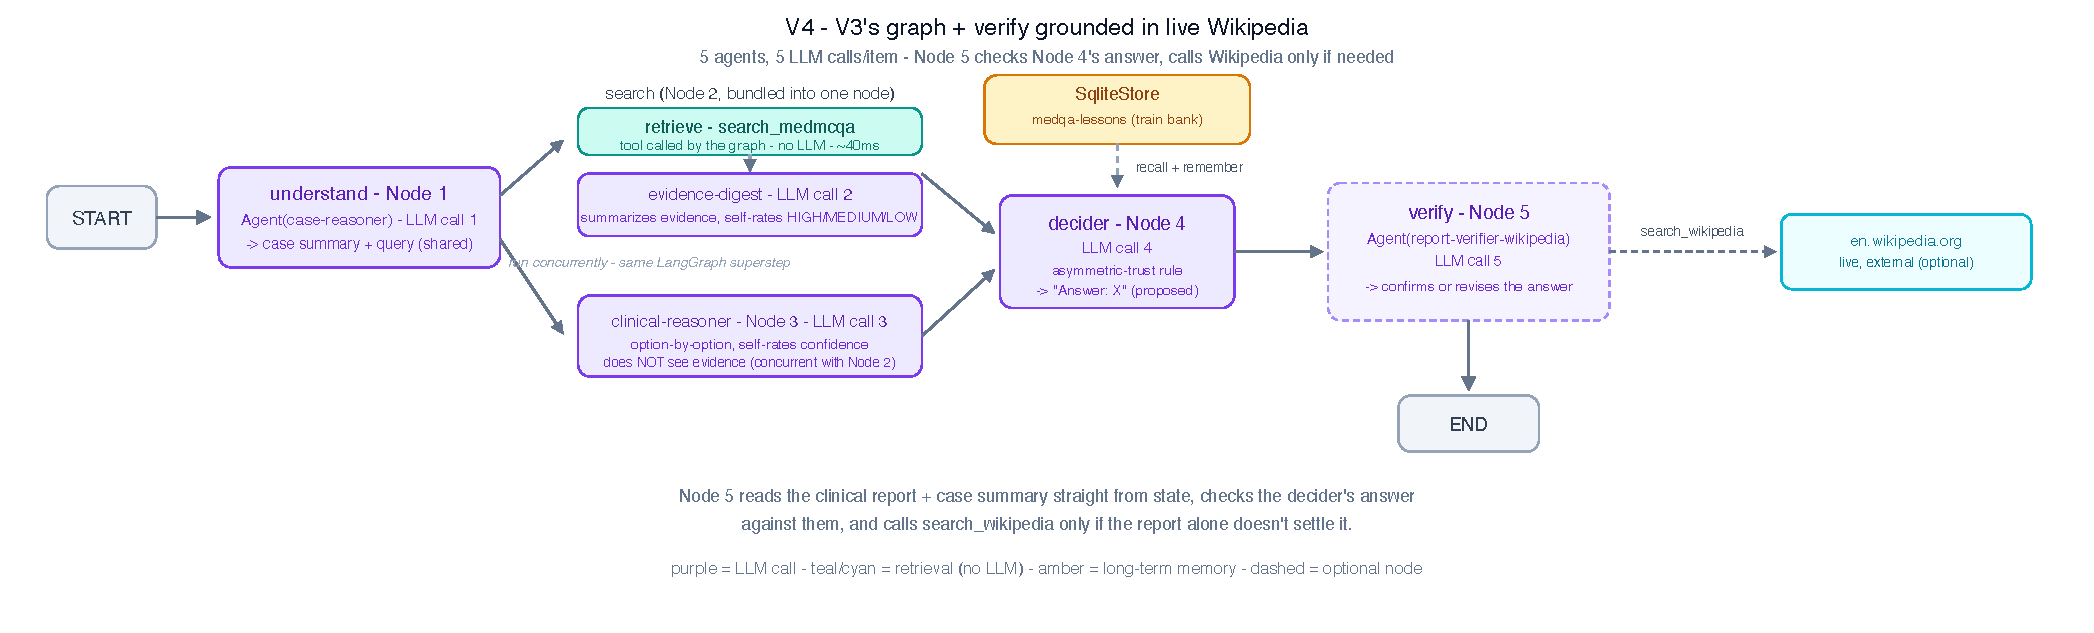
\includegraphics[width=\textwidth]{v4_flow.pdf}
  \caption{V4: đồ thị V3 + Node~5 (\texttt{report-verifier-wikipedia}), audit đáp án và gọi
  \texttt{search\_wikipedia} khi cần.}
  \label{fig:v4}
\end{figure}

\paragraph{V5 - V3 + bộ kiểm chứng đọc dùng lại các ca đã sai.} V5 thêm CÙNG Node~5 của V4
nhưng không gọi Wikipedia; thay vào đó nó \texttt{recall} từ một kho dữ liệu \emph{riêng biệt} với kho chung
của V3 - \textbf{kho tiến hoá} (\texttt{medqa-mistakes}), chỉ chứa bài học từ những câu hệ thống từng
trả lời SAI (\S\ref{sec:memory}). Bộ kiểm chứng không bao giờ biết đáp án đúng của câu đang xử lý -
nó chỉ đọc bài học đã đúc kết từ những câu KHÁC, tương tự về chủ đề. V5 thêm \textbf{Node~6 -
\texttt{distill\_mistake}}, chạy SAU \texttt{verify}: đây là nút DUY NHẤT trong toàn đồ thị đọc đáp án
đúng (\texttt{item.answer\_idx}) - nếu đáp án cuối cùng SAI, nó gọi một tác tử \texttt{mistake-analyst}
(được cho biết đáp án đúng) để đúc kết một bài học sửa sai, rồi ghi vào kho tiến hoá cho các câu
tương lai; nếu đáp án ĐÚNG, nó không làm gì.

\begin{figure}[tbp]
  \centering
  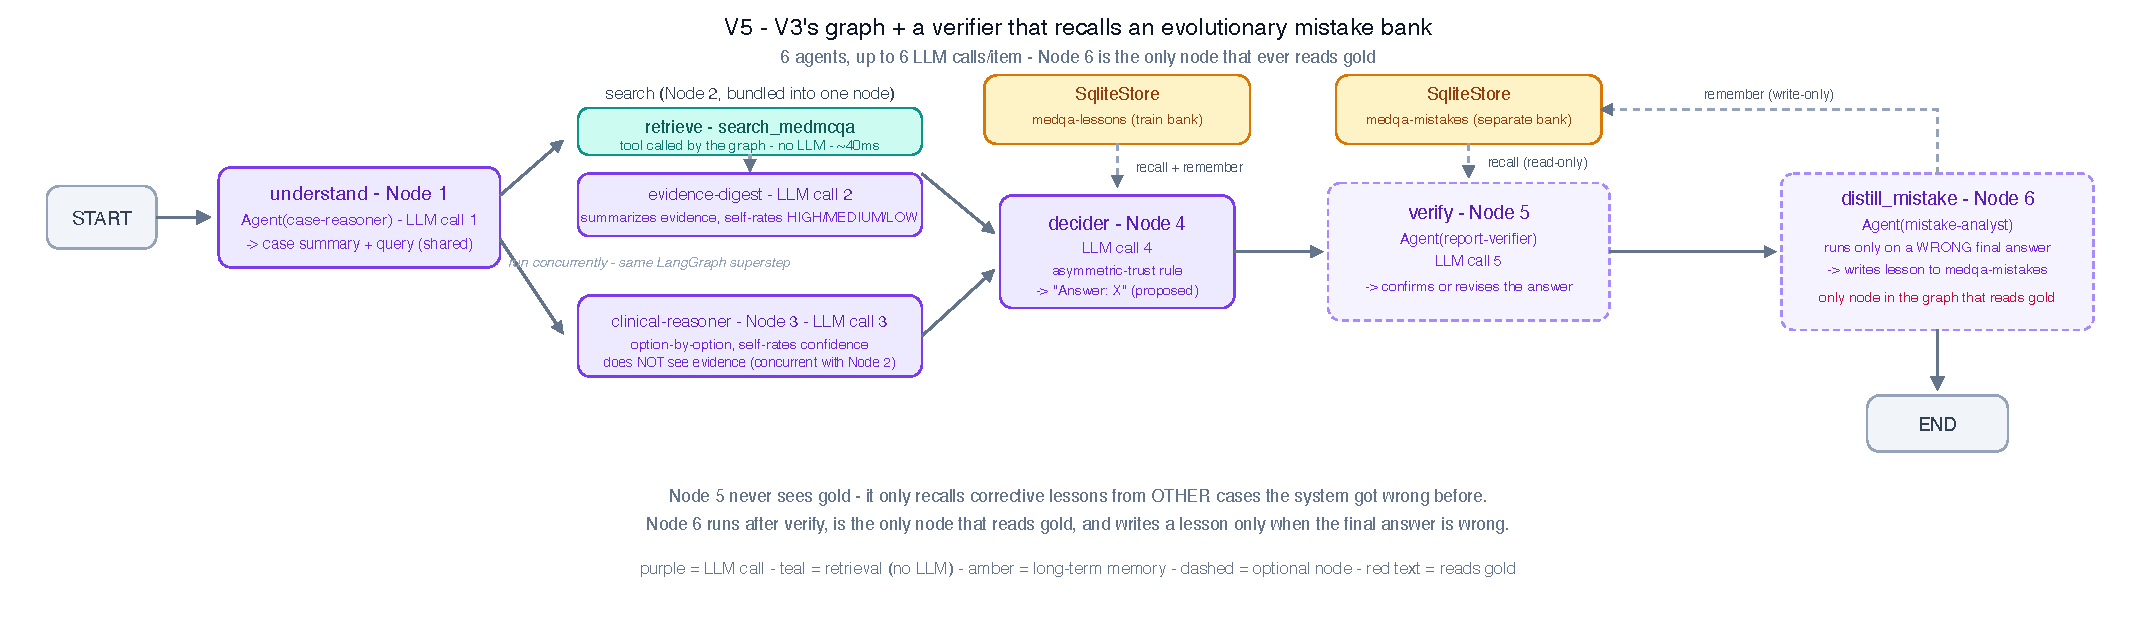
\includegraphics[width=\textwidth]{v5_flow.pdf}
  \caption{V5: đồ thị V3 + Node~5 (đọc \texttt{medqa-mistakes}) + Node~6
  \texttt{distill\_mistake}, chỉ ghi khi đáp án sai.}
  \label{fig:v5}
\end{figure}

\FloatBarrier
\subsection{Thiết kế RAG}
\label{sec:rag}
Toàn hệ thống dùng chung một \emph{nguồn dữ liệu} và một \emph{embedder} truy hồi.

\begin{enumerate}[nosep]
  \item \textbf{Dữ liệu.} \textbf{MedMCQA}~\cite{pal2022medmcqa} (182.822 câu thi đã giải kèm đáp án
  và giải thích) là dữ liệu truy hồi \emph{duy nhất}, dùng cho toàn bộ V1-V5 - tức truy hồi các ví dụ
  mẫu đã giải (tương tự Medprompt~\cite{nori2023medprompt}), không phải văn bản tham khảo. Chỉ phần
  câu hỏi được nhúng; đáp án và giải thích nằm trong metadata.
  \item \textbf{Embedder.} Một embedder duy nhất: \texttt{qwen3-embedding:4b} (ngữ cảnh 32K token,
  chạy qua Ollama), được áp dụng cho cả toàn bộ V2-V5.
  \item \textbf{Vector Database.} ChromaDB, một collection duy nhất
  (\texttt{knowledge\_medmcqa\_qwen3}), đo độ phù hợp bằng cosine similarity.
  \item \textbf{Cơ chế truy hồi.} \texttt{search\_medmcqa} trả về $k{=}5$ câu thi gần nhất kèm đáp án
  và giải thích (định dạng \texttt{Q:/A:/Why:}).
  \item \textbf{Đánh giá độ liên quan bằng nhãn.} Hệ thống tự đánh giá độ liên quan
  của bằng chứng vừa truy hồi bằng một nhãn HIGH/MEDIUM/LOW, không so điểm cosine với một ngưỡng cố
  định ở bất kỳ đâu.
  \item \textbf{Tối ưu truy vấn (query reformulation).} Nếu độ liên quan bị đánh giá LOW,
  viết lại một truy vấn tìm kiếm mới bằng cách thêm ngữ cảnh (context) từ tình huống, rồi truy hồi lại.
  \item \textbf{Luật quyết định: tin cậy bất đối xứng.} Một luật dùng chung cho bước chốt đáp án của V1
  và Node~4 (\texttt{decider}, V2-V5). Nếu bằng chứng được chấm HIGH và nghiêng rõ về một phương án,
  phương án đó là đáp án mặc định; chỉ bị lật lại khi tình huống có một dấu hiệu \emph{cụ thể} mà bằng
  chứng đã bỏ sót hoặc hiểu sai, không phải một cảm giác chung chung là ``có lẽ khác''. Nếu bằng chứng
  chỉ MEDIUM/LOW hoặc không có, nó bị bỏ qua hoàn toàn và đáp án chọn thuần từ lập luận lâm sàng, đúng
  như cách V0 quyết định.
\end{enumerate}

\begin{figure}[h]
  \centering
  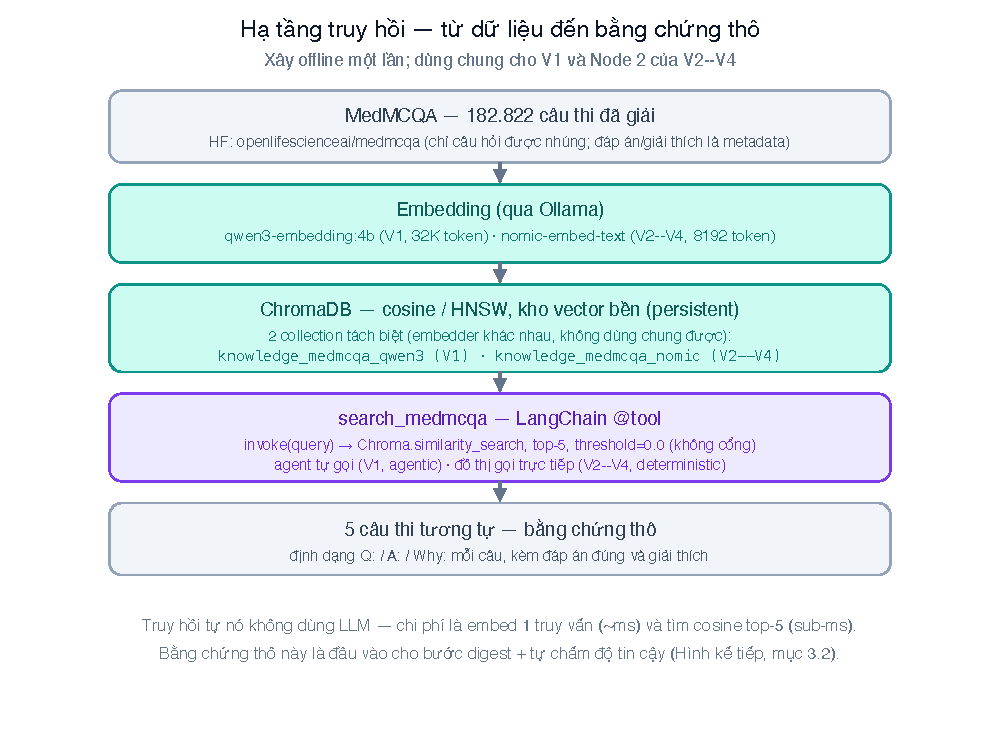
\includegraphics[width=0.75\textwidth]{rag_infra.pdf}
  \caption{Hạ tầng truy hồi: MedMCQA $\rightarrow$ embedding $\rightarrow$ ChromaDB $\rightarrow$
  \texttt{search\_medmcqa}.}
  \label{fig:rag-infra}
\end{figure}

\begin{figure}[h]
  \centering
  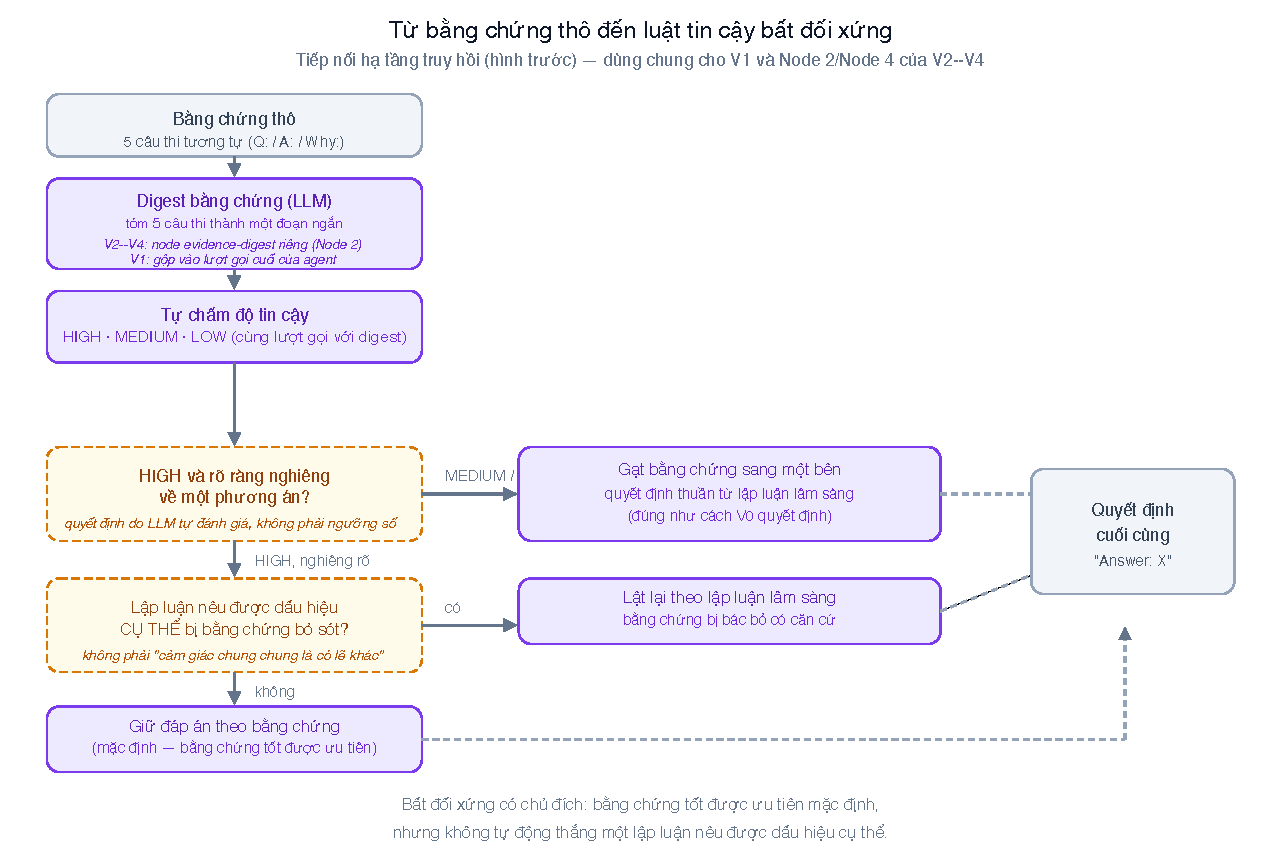
\includegraphics[width=0.8\textwidth]{rag_design.pdf}
  \caption{Từ bằng chứng thô đến luật tin cậy bất đối xứng, dùng chung cho V1 và Node~4
  (\texttt{decider}).}
  \label{fig:rag-design}
\end{figure}

\FloatBarrier
\subsection{Thiết kế bộ nhớ}
\label{sec:memory}
\paragraph{Bộ nhớ ngắn hạn (trong một câu hỏi).} Dựa thẳng vào \texttt{state}: mỗi biến thể chạy trên
cùng một \texttt{StateGraph(QAState)} (\texttt{graph/build.py}), và \texttt{QAState} (một
\texttt{TypedDict}, \texttt{graph/state.py}) chính là bộ nhớ ngắn hạn - mỗi nút ghi ra một vài trường
(\texttt{case\_understanding}, \texttt{evidence}, \texttt{clinical\_report}, ...), nút chạy sau đọc
thẳng từ đó, không cần một tác tử/kho bộ nhớ riêng. Mặc định mọi biến thể (V0-V5) đều có nó:
khác biệt giữa các biến thể chỉ là số nút, và do đó số trường tồn tại trong hệ thống.
(Bảng~\ref{tab:variants}).

\begin{table}[h]
  \centering
  \caption{Short-term memory: each \texttt{QAState} field is a channel from one node to the next.}
  \label{tab:memory-design}
  \small
  \begin{tabular}{@{}p{0.24\textwidth}p{0.20\textwidth}p{0.46\textwidth}@{}}
    \toprule
    Trường trong QAState & Ghi bởi & Đọc bởi \\
    \midrule
    \texttt{query} & Node 1 (understand) & Node 2 (search) \\[3pt]
    \texttt{evidence} & Node 2 (search) & Node 4 (decider), Node 5 (verifier) \\[3pt]
    \texttt{clinical\_report} & Node 3 (reasoning) & Node 4 (decider), Node 5 (verifier) \\[3pt]
    \texttt{case\_understanding} & Node 1 (understand) & Node 3 (reasoning), Node 5 (verifier) \\[3pt]
    \texttt{answer, rationale} & Node 4 (decider) & overwritten by Node 5, if present (V4/V5); Node 6 reads \texttt{answer} to check correctness (V5) \\
    \bottomrule
  \end{tabular}
\end{table}

\paragraph{Bộ nhớ dài hạn (episodic, sử dụng qua nhiều câu hỏi): hai kho tách biệt.} Cả hai dùng chung một
\texttt{SqliteStore} của LangGraph (\texttt{data/longterm/lessons.sqlite},
\texttt{graph/longterm.py}), phân biệt bằng namespace:
\begin{itemize}[nosep]
  \item \textbf{Kho chung} (\texttt{medqa-lessons}, V3-V5): \texttt{decider} (Node~4) \texttt{recall}
  bài học từ những câu TƯƠNG TỰ đã gặp trước - xếp hạng bằng số từ chủ đề trùng nhau (không phải
  embedding, để giữ chi phí thấp và không cần một collection thứ hai) - rồi \texttt{remember} một bài
  học sau khi chốt, cho mọi câu, đúng lẫn sai.
  \item \textbf{Kho tiến hoá} (\texttt{medqa-mistakes}, V5): chỉ chứa bài học từ những câu hệ thống
  từng trả lời sai. Bộ kiểm chứng (Node~5) chỉ \texttt{recall} từ kho này, không bao giờ ghi và không
  bao giờ thấy đáp án đúng; Node~6 (\texttt{distill\_mistake}), chạy sau Node~5, là nút duy nhất đọc
  đáp án đúng, và chỉ ghi một bài học khi đáp án cuối cùng sai (\S\ref{sec:variants}).
\end{itemize}
\textbf{Chống rò rỉ dữ liệu (contamination).} Rủi ro là: bài học của câu thứ $N$ đang được chấm rò
sang câu thứ $N{+}k$ trong CÙNG lượt chấm đó, làm tăng ảo độ chính xác vì lý do không liên quan tới
chất lượng lập luận. Lớp bảo vệ đang có là \emph{namespace}: mỗi kho gồm cả tên \emph{split}, nên bài
học học trên \texttt{train} là vô hình khi truy vấn namespace \texttt{test}.

\begin{figure}[tbp]
  \centering
  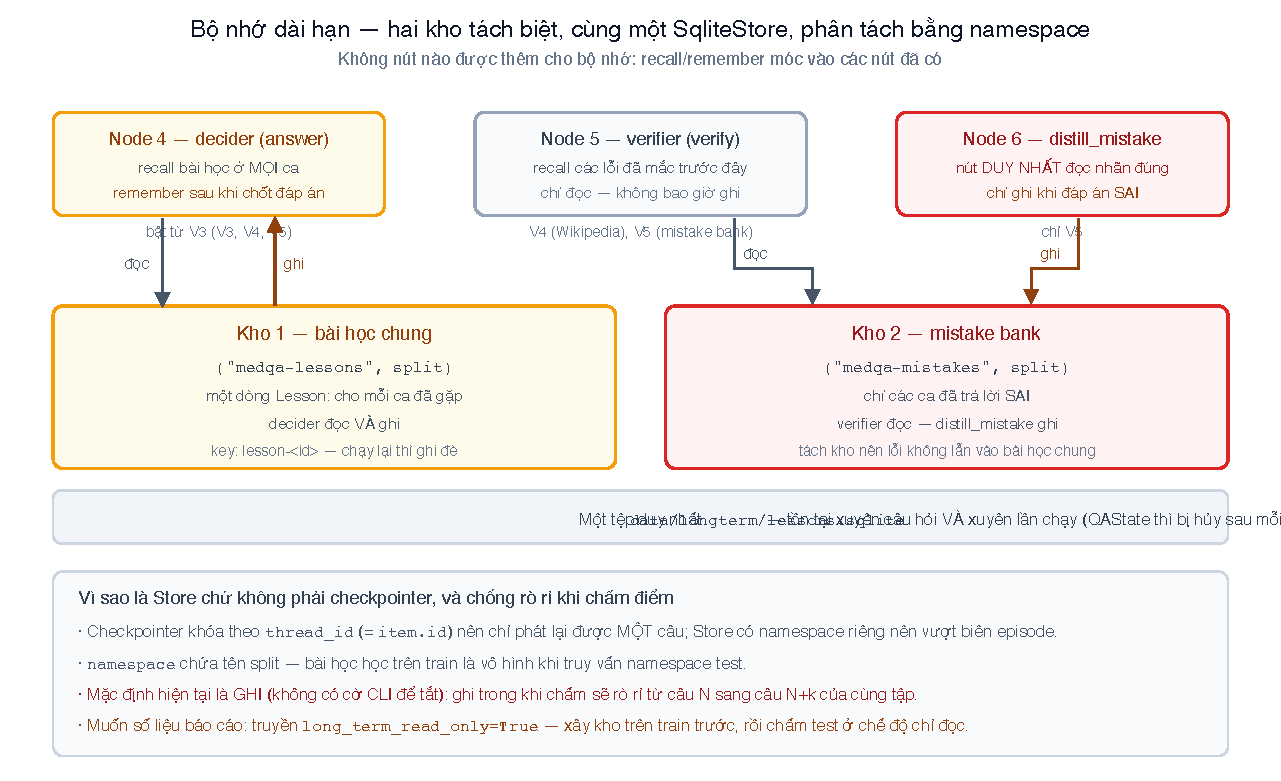
\includegraphics[width=0.95\textwidth]{longterm_memory.pdf}
  \caption{Bộ nhớ dài hạn: hai kho tách biệt bằng namespace trong một \texttt{SqliteStore};
  \texttt{decider} đọc/ghi kho chung, bộ kiểm chứng chỉ đọc kho lỗi.}
  \label{fig:longterm-memory}
\end{figure}

\FloatBarrier
\subsection{Thiết kế bộ kiểm chứng}
\label{sec:verifier}
V4 và V5 dùng chung một Node~5 (\texttt{report-verifier}), chạy ngay sau khi \texttt{decider} chốt
đáp án. Hai biến thể chỉ khác nhau ở một điểm: nguồn bằng chứng bổ sung mà Node~5 tra cứu khi báo cáo của
Node~3 chưa đủ rõ để quyết.
\begin{itemize}[nosep]
  \item \textbf{V4 - tra Wikipedia trực tuyến.} Gọi công cụ \texttt{search\_wikipedia} qua MediaWiki
  API, có timeout; nếu mạng lỗi, nó trả về chuỗi rỗng và hệ thống suy biến về đúng hành vi của V3, chứ
  không làm hỏng lượt chạy. Đây là nguồn bằng chứng độc lập đầu tiên trong toàn hệ thống không bắt
  nguồn từ MedMCQA. Chọn Wikipedia thay vì tìm kiếm chung trên internet vì Wikipedia
  chỉ có nội dung bách khoa về y khoa (bệnh, thuốc, cơ chế...), không thể vô tình lộ đáp án của một câu
  hỏi thi cụ thể như một trang đề thi hay diễn đàn giải đề có thể làm.
  \item \textbf{V5 - tra lại kho các câu từng trả lời sai.} Gọi \texttt{recall\_mistakes} để đọc từ kho
  \texttt{medqa-mistakes} (\S\ref{sec:memory}) bài học rút ra từ những câu tương tự mà hệ thống từng
  trả lời sai trước đó. Bộ kiểm chứng ở đây không có công cụ tra cứu nào khác ngoài kho này, và chỉ
  đọc: nó không bao giờ ghi, và không bao giờ thấy đáp án đúng của câu đang xử lý.
\end{itemize}

V5 có thêm một nút mà V4 không có: \textbf{Node~6 - \texttt{distill\_mistake}}, chạy ngay sau Node~5.
Đây là nút duy nhất trong toàn đồ thị được phép đọc đáp án đúng (\texttt{item.answer\_idx}). Nếu đáp án
cuối cùng đúng, nó không làm gì cả, không tốn thêm lượt gọi LLM nào. Nếu sai, nó gọi riêng một tác tử
(\texttt{mistake-analyst}), cho biết cả đáp án hệ thống vừa chọn lẫn đáp án đúng, để rút ra một bài học
sửa sai rồi ghi vào kho tiến hoá cho những câu hỏi khác đọc lại về sau. Nút này không bao giờ được phép
sửa đáp án của câu đang xử lý - việc của nó chỉ là để lại bài học cho lần sau, không phải ảnh hưởng
điểm số của câu hiện tại.

% =====================================================================
\FloatBarrier
\section{Thiết lập thực nghiệm}
\label{sec:setup}
% =====================================================================

\subsection{Cấu trúc mã nguồn}
\label{sec:reposcructure}
Toàn bộ mã nguồn nằm dưới \texttt{src/agent\_hospital/}, chia theo nhiệm vụ - mỗi thư mục con một mối
quan tâm riêng (đồ thị LangGraph, tác tử, truy hồi, đánh giá):

\begin{lstlisting}
src/agent_hospital/
  __main__.py       CLI: chay mot bien the tren MedQA-USMLE, in ra metric
  config.py         RunConfig/RagConfig - noi tap trung moi tuy chinh
  models.py         provider:model -> BaseChatModel, khong phu thuoc nha cung cap
  roles.py          registry system prompt (9 vai, xem bang tom tat o 4.2)
  predict.py        chay mot bien the, ghi du doan tung cau ra .jsonl
  evaluate.py       tinh metric tu cac file du doan

  agents/
    base.py         Agent - lop boc create_agent cua LangChain, khoi tao tre

  graph/
    state.py        QAState - trang thai dung chung truyen qua moi node
    build.py        RunConfig -> StateGraph da compile
    nodes.py        cac node dung lai duoc (state -> partial state)
    longterm.py     bo nho dai han: hai kho trong mot SqliteStore

  qa/
    variants.py     cac preset V0-V5 + diem vao build_variant
    mcq.py          dung prompt cho cau hoi, trich dap an
    metrics.py      do luong tung cau + so sanh giua bien the
    reasoning.py    tac tu rut gon truy van (V1)

  knowledge/
    embeddings.py   ham embedding cho kho tri thuc RAG (Ollama)
    ingest.py       nap MedMCQA vao Chroma
    retriever.py    truy hoi cosine top-k tren Chroma
    wikipedia.py    tim Wikipedia truc tuyen (nguon cua bo kiem chung V4)

  diseases/
    medqa_usmle.py  nap tap MedQA-USMLE (split dung de cham diem)
\end{lstlisting}

Quy ước xuyên suốt: mỗi \texttt{RunConfig} (\texttt{config.py}) là toàn bộ tham số của một lượt chạy;
\texttt{qa/variants.py} chỉ định nghĩa SÁU preset cụ thể (V0-V5) từ đúng một \texttt{RunConfig}, không
có nhánh rẽ nào khác trong \texttt{graph/build.py} ngoài những cờ mà \texttt{RunConfig} khai báo.

\subsection{Mô hình và prompt}
Mô hình trả lời mặc định là \textbf{Qwen2.5}~\cite{qwen2025} (Ollama, có gọi công cụ): \texttt{qwen2.5:7b}
cho mọi biến thể và mọi con số được báo cáo. Mọi vai chạy ở \textbf{temperature~0}: ở temperature mặc định, chênh
lệch $V1-V0$ dao động giữa các lần chạy lớn hơn cả bản thân hiệu ứng, nên tính tất định là bắt buộc để
McNemar ghép cặp có ý nghĩa. Các nhà cung cấp đám mây (\texttt{anthropic:}, \texttt{openai:},
\texttt{google:}, \texttt{openrouter:}) được hỗ trợ qua cùng một đặc tả \texttt{provider:model}.

Toàn hệ thống có 9 vai (\texttt{roles.py:ROLE\_PROMPTS}), mỗi vai một system prompt riêng, dùng nguyên
văn tiếng Anh (prompt vận hành thực tế). Bảng~\ref{tab:roles} tóm tắt việc của từng vai; nội dung đầy đủ
nằm trong mã nguồn. Node 1-4 xuất hiện ở mọi biến thể V2-V5 (\S\ref{sec:variants}).

\begin{table}[h]
  \centering
  \caption{Tóm tắt system prompt của 9 vai trong hệ thống.}
  \label{tab:roles}
  \small
  \begin{tabular}{@{}p{0.30\textwidth}p{0.14\textwidth}p{0.46\textwidth}@{}}
    \toprule
    Vai (\texttt{roles.py}) & Dùng ở & Tóm tắt \\
    \midrule
    \texttt{baseline} & V0 & Trả lời trực tiếp từ kiến thức riêng. \\[3pt]
    \texttt{rag-agent} & V1 & Tự hiểu ca, tìm kiếm, lập luận, quyết định. \\[3pt]
    \texttt{case-reasoner} & Node 1 & Tóm ca bệnh, viết truy vấn tìm kiếm. \\[3pt]
    \texttt{clinical-reasoner} & Node 3 & Lập luận option-by-option, tự chấm tin cậy. \\[3pt]
    \texttt{evidence-digest} & Node 2 & Tóm bằng chứng, tự chấm tin cậy. \\[3pt]
    \texttt{decider} & Node 4 & Tổng hợp báo cáo + bằng chứng, chốt đáp án. \\[3pt]
    \texttt{report-verifier} & Node 5 (V5) & Soát đáp án; tra thêm kho câu từng sai. \\[3pt]
    \texttt{report-verifier-wikipedia} & Node 5 (V4) & Soát đáp án; tra thêm Wikipedia. \\[3pt]
    \texttt{mistake-analyst} & Node 6 (V5) & Chỉ chạy khi sai: đúc kết một bài học. \\
    \bottomrule
  \end{tabular}
\end{table}

\texttt{parse\_choice} trích đáp án từ \texttt{Answer: X} hoặc \texttt{answer is X} (không phân biệt hoa
thường), dự phòng bằng chữ cái \texttt{A|B|C|D} độc lập đầu tiên; phản hồi không trích được trả về
\texttt{None} và bị tính là \emph{không hợp lệ}, không bao giờ bị tính nhầm thành câu trả lời sai. Tỷ lệ không
hợp lệ đo được là \textbf{0.0\%} xuyên suốt.

\subsection{Phần cứng / thiết lập API}
\begin{itemize}[nosep]
  \item \textbf{Phần cứng:} chạy trên một máy cá nhân, chạy các dịch vụ cục bộ.
  \item \textbf{Dữ liệu:} \texttt{openlifescienceai/medqa} (train 10{,}178 / validation 1{,}272 /
  \textbf{test 1{,}273}), lưu cache cục bộ và nạp không cần mạng.
\end{itemize}

Lệnh \texttt{predict} và \texttt{evaluate} cho từng biến thể:

\begin{lstlisting}
PYTHONPATH=src .venv/bin/python -m agent_hospital.predict -v V0 -s test -m qwen2.5:7b
PYTHONPATH=src .venv/bin/python -m agent_hospital.predict -v V1 -s test -m qwen2.5:7b
PYTHONPATH=src .venv/bin/python -m agent_hospital.predict -v V2 -s test -m qwen2.5:7b
PYTHONPATH=src .venv/bin/python -m agent_hospital.predict -v V3 -s test -m qwen2.5:7b
PYTHONPATH=src .venv/bin/python -m agent_hospital.predict -v V4 -s test -m qwen2.5:7b
PYTHONPATH=src .venv/bin/python -m agent_hospital.predict -v V5 -s test -m qwen2.5:7b

PYTHONPATH=src .venv/bin/python -m agent_hospital.evaluate --dir data/eval_runs --baseline V0
\end{lstlisting}
\texttt{predict.py} ghi dự đoán từng câu vào \texttt{data/eval\_runs/<variant>\_<split>\_<model>.jsonl}
kèm một tệp \texttt{.meta.json} (cấu hình lượt chạy); chạy lại cùng lệnh sẽ RESUME - bỏ qua những câu
đã có trong tệp, chỉ chấm tiếp các câu còn thiếu, an toàn nếu lượt chạy trước bị ngắt giữa chừng.
\texttt{evaluate.py} đọc mọi tệp \texttt{.jsonl} trong \texttt{--dir} và in ra bảng leaderboard (độ
chính xác, khoảng tin cậy bootstrap, tỷ lệ không hợp lệ) cùng bảng so sánh ghép cặp với
\texttt{--baseline}.



% =====================================================================
\FloatBarrier
\section{Kết quả đánh giá}
\label{sec:results}
% =====================================================================
Chỉ số chính là độ chính xác, $\text{Độ chính xác} = (\text{số dự đoán đúng}) / (\text{số câu hỏi})$.
Nhóm báo cáo thêm tỷ lệ phản hồi không hợp lệ, mức tăng độ chính xác so với V0, Thắng/Thua/Hòa so với
baseline, khoảng tin cậy bootstrap 95\%, kiểm định ghép cặp McNemar, độ trễ và số token.

\paragraph{Trạng thái đo lường.} Mục này báo cáo một lần chạy trên \textbf{150 câu đầu của tập test}
($n{=}150$/1273, qwen2.5:7b, temperature~0) cho cả sáu biến thể V0-V5 - cùng 150 câu, cùng thứ tự (xác
nhận bằng \texttt{item\_id}), nên so sánh chéo giữa mọi biến thể đều hợp lệ.
\todo{Đang chạy tiếp V3-V5 lên $n{=}300$; sẽ cập nhật mục này, rồi tiến tới $n{=}1273$ cho số liệu
chính thức. $n{=}150$ đủ lớn để McNemar có ý nghĩa cho V2-V5 so với V0, nhưng chưa đủ để phân biệt
V3/V4/V5 với V2 (xem dưới) - một hiệu ứng thật nhưng nhỏ có thể chưa lộ ra ở quy mô này.}

\subsection{Bảng chính (main board): 150 câu đầu của tập test, qwen2.5:7b}
\begin{table}[h]
  \centering
  \caption{Kết quả trên 150 câu đầu của tập test, qwen2.5:7b, temperature~0.}
  \label{tab:official}
  \small
  \begin{tabular}{@{}p{0.20\textwidth}cccrr@{}}
    \toprule
    Variant & Accuracy & 95\% Bootstrap CI & Invalid & Latency/query & Tokens/query \\
    \midrule
    V0: LLM trực tiếp & 0.627 (94/150) & [0.553, 0.707] & 0.0\% & 1.71\,s & 495 \\
    V1: RAG-only (agentic) & 0.633 (95/150) & [0.553, 0.713] & 0.0\% & 5.40\,s & 2894 \\
    V2: Đa tác tử (4 nút) & \textbf{0.720} (108/150) & [0.647, 0.793] & 0.0\% & 19.18\,s & 4418 \\
    V3: V2 + bộ nhớ dài hạn & \textbf{0.720} (108/150) & [0.647, 0.787] & 0.0\% & 21.22\,s & 4620 \\
    V4: V3 + bộ kiểm chứng Wikipedia & 0.707 (106/150) & [0.633, 0.780] & 0.0\% & 24.15\,s & 6357 \\
    V5: V3 + bộ kiểm chứng kho tiến hoá & 0.713 (107/150) & [0.640, 0.780] & 0.0\% & 25.85\,s & 6471 \\
    \bottomrule
  \end{tabular}
\end{table}
Tỷ lệ không hợp lệ là \textbf{0.0\% ở cả sáu biến thể}. V1 nhỉnh hơn V0 một chút ($+0.7$ điểm, không có
ý nghĩa thống kê - xem McNemar dưới), nhất quán với mọi lần đo retrieval-only trong dự án: truy hồi
riêng không giúp ích trên MedQA. V2 và V3 \textbf{đồng cao nhất} ($+9.3$ điểm so với V0); V4 và V5 thấp
hơn một chút ($+8.0$ và $+8.7$ điểm) nhưng vẫn cao hơn V0 rõ rệt - chênh lệch giữa V2/V3/V4/V5 với nhau
nằm trong nhiễu của mẫu (xem McNemar dưới).

\subsection{So sánh với baseline (so sánh ghép cặp)}
\begin{table}[h]
  \centering
  \caption{So sánh ghép cặp trên 150 câu đầu của tập test, qwen2.5:7b. Tính trực tiếp từ bản ghi từng câu.}
  \label{tab:paired}
  \small
  \begin{tabular}{@{}p{0.42\textwidth}cc c@{}}
    \toprule
    Comparison & Delta & W/L/T & McNemar $p$ \\
    \midrule
    V1 vs V0 & $+0.7$ điểm & 15/14/121 & $1.000$ (không ý nghĩa) \\
    \textbf{V2 vs V0} & $\mathbf{+9.3}$ \textbf{điểm} & \textbf{20/6/124} & $\mathbf{0.0094}$ \textbf{(có ý nghĩa)} \\
    \textbf{V3 vs V0} & $\mathbf{+9.3}$ \textbf{điểm} & \textbf{21/7/122} & $\mathbf{0.0125}$ \textbf{(có ý nghĩa)} \\
    \textbf{V4 vs V0} & $\mathbf{+8.0}$ \textbf{điểm} & \textbf{19/7/124} & $\mathbf{0.0290}$ \textbf{(có ý nghĩa)} \\
    \textbf{V5 vs V0} & $\mathbf{+8.7}$ \textbf{điểm} & \textbf{20/7/123} & $\mathbf{0.0192}$ \textbf{(có ý nghĩa)} \\
    V3 vs V2 (hiệu ứng bộ nhớ dài hạn) & $+0.0$ điểm & 4/4/142 & $1.000$ (không ý nghĩa) \\
    V4 vs V2 (hiệu ứng kiểm chứng Wikipedia) & $-1.3$ điểm & 3/5/142 & $0.727$ (không ý nghĩa) \\
    V5 vs V2 (hiệu ứng kiểm chứng kho tiến hoá) & $-0.7$ điểm & 5/6/139 & $1.000$ (không ý nghĩa) \\
    V4 vs V3 (tách riêng đúng một bộ kiểm chứng) & $-1.3$ điểm & 4/6/140 & $0.754$ (không ý nghĩa) \\
    V5 vs V3 (tách riêng đúng một bộ kiểm chứng) & $-0.7$ điểm & 5/6/139 & $1.000$ (không ý nghĩa) \\
    \bottomrule
  \end{tabular}
\end{table}

\subsection{Phân tích Thắng/Thua/Hòa}
Cột T/T/H đếm theo từng câu: biến thể sửa được lỗi của baseline (thắng), làm hỏng một câu baseline vốn
đúng (thua), hay trùng khớp (hòa). \textbf{V2 vs V0}: 20 thắng so với 6 thua - V2 sửa được hơn gấp ba
số câu nó làm hỏng, và với 26 câu bất đồng, McNemar cho $p{=}0.0094$: cải thiện có ý nghĩa thống kê.
\textbf{V3, V4, V5 vs V0}: cùng mẫu hình - đều thắng rõ rệt so với thua (21/7, 19/7, 20/7), đều có ý
nghĩa thống kê ($p{<}0.03$ cho cả ba). \textbf{Nhưng so với V2}: cả ba đều KHÔNG khác biệt có ý nghĩa
(mọi $p{\geq}0.73$) - trên 150 câu này, chưa có bằng chứng rằng bộ nhớ dài hạn (V3) hay một trong hai
thiết kế bộ kiểm chứng (V4, V5) cải thiện thêm so với riêng kiến trúc đa tác tử của V2. Đây là phát
hiện ngược với kỳ vọng ban đầu của Nhóm, và được báo cáo trung thực thay vì diễn giải có lợi cho thiết
kế.

\subsection{Chi phí và độ trễ}
Chi phí đo bằng \emph{độ trễ} và \emph{số token} (đầu vào + đầu ra) cho mô hình cục bộ (không có phí
API). V0: \textbf{1.71\,s/câu}, \textbf{495 token/câu}. V1 (agentic): \textbf{5.40\,s/câu}
($\sim$3$\times$ V0), \textbf{2894 token/câu} ($\sim$6$\times$ V0) - vòng lặp gọi công cụ sinh nhiều
token hơn một lượt trả lời trực tiếp. V2 (4 nút): \textbf{19.18\,s/câu} ($\sim$11$\times$ V0),
\textbf{4418 token/câu} - bốn tác tử, một số nút chạy tuần tự, nên chi phí cộng dồn theo số lượt gọi
LLM. V3 (V2 + bộ nhớ dài hạn, vẫn 4 nút): \textbf{21.22\,s/câu}, \textbf{4620 token/câu} - chậm hơn V2
dù không thêm nút hay lượt gọi LLM nào, chỉ hai lần đọc/ghi kho \texttt{SqliteStore} thêm quanh lượt
gọi \texttt{decider} sẵn có. V4 (V3 + bộ kiểm chứng Wikipedia): \textbf{24.15\,s/câu} ($\sim$3\,s hơn
V3), \textbf{6357 token/câu} - chi phí của Node~5, gồm cả những lần thật sự gọi
\texttt{search\_wikipedia}. V5 (V3 + bộ kiểm chứng kho tiến hoá): \textbf{25.85\,s/câu}, \textbf{6471
token/câu} - thêm cả Node~5 lẫn Node~6 (\texttt{distill\_mistake}, chỉ tốn lượt gọi LLM khi đáp án
cuối cùng sai). Vì cả bộ nhớ dài hạn lẫn hai thiết kế bộ kiểm chứng đều chưa cho thấy cải thiện độ
chính xác đáng kể ở quy mô này, chi phí thêm $\sim$10-35\% độ trễ và token của V3-V5 so với V2 hiện
chưa được biện minh bằng bằng chứng - một điểm cần theo dõi khi đo ở quy mô lớn hơn.

% =====================================================================
\FloatBarrier
\section{Phân tích lỗi}
\label{sec:error}
% =====================================================================
Mục này dùng tệp dự đoán từng câu của V0-V3 (\texttt{data/eval\_runs/*.jsonl}, $n{=}300$, xem
\S\ref{sec:results}) - không còn chỉ là mô tả định tính.

Tỷ lệ không hợp lệ là 0.0\% trên cả bốn biến thể, nên mọi lỗi đều là chọn sai lựa chọn thực sự, không
phải lỗi trích xuất. Hai mẫu hình hiện rõ trong dữ liệu ghép cặp:
\begin{itemize}[nosep]
  \item \textbf{Câu trung tính với truy hồi.} V1 vs V0: 29 thắng, 34 thua, 237 hòa (\S\ref{sec:results})
  - trên đa số câu (79\%), truy hồi không đổi đáp án, nhất quán với việc MedQA chủ yếu đòi hỏi lập
  luận chứ không phải tra cứu dữ kiện.
  \item \textbf{Câu nhạy với cấu trúc lập luận.} V2 vs V1: 48 thắng, 27 thua (\S\ref{sec:results}) -
  tách hiểu ca bệnh / tìm kiếm / lập luận / quyết định thành bốn nút làm đổi quyết định trên nhiều câu
  hơn hẳn so với chênh lệch do riêng truy hồi gây ra, khu trú phần lớn mức tăng vào khâu cấu trúc lập
  luận chứ không phải bằng chứng truy hồi (vẫn cùng một nguồn MedMCQA).
\end{itemize}

\begin{table}[h]
  \centering
  \caption{Phân tích lỗi với ví dụ thật từ tệp dự đoán $n{=}300$ (V0 vs V2).}
  \label{tab:error}
  \small
  \begin{tabular}{@{}p{0.26\textwidth}p{0.11\textwidth}p{0.53\textwidth}@{}}
    \toprule
    Loại lỗi & Mã câu & Ghi chú \\
    \midrule
    V2 lập luận chi tiết nhưng chốt sai, trong khi V0 (một lượt) tình cờ đúng &
    \texttt{test-00012} &
    V0 chọn đúng (B); Node~3 của V2 xây một chuỗi lập luận cụ thể dẫn tới u xơ thần kinh loại 2, decider
    theo lập luận đó và chọn D (sai). \\
    Bị phương án nghe hợp lý nhưng sai đánh lừa &
    \texttt{test-00013} &
    V0 chọn đúng (D, sa van hai lá); V2 lập luận nghiêng về bệnh cơ tim phì đại tắc nghẽn (HOCM) và
    chọn A (sai) - một chẩn đoán phân biệt hợp lý nhưng không khớp đặc điểm tiếng thổi trong đề bài. \\
    V2 sửa đúng nhờ tri thức chuyên biệt hơn &
    \texttt{test-00003} &
    V0 chọn sai (B, nhiễm khuẩn vùng chậu); Node~3 của V2 xác định đúng đặc điểm vi khuẩn học (khuẩn lạc
    hồng trên môi trường MacConkey) và chọn D (đúng). \\
    V2 sửa đúng nhờ bám sát đúng câu hỏi được hỏi &
    \texttt{test-00024} &
    V0 chọn sai (B, tràn khí màng phổi áp lực); V2 nhận ra câu hỏi thực sự là bước xử trí tiếp theo chứ
    không phải chẩn đoán, chọn A (đặt nội khí quản, đúng). \\
    \bottomrule
  \end{tabular}
\end{table}
\todo{Bảng trên mới liệt kê 4 ví dụ minh hoạ, chưa phải phân loại lỗi có hệ thống trên toàn bộ các câu
bất đồng; có thể mở rộng bằng cách phân loại tự động (vd.\ LLM-judge) trên tệp dự đoán khi có thời
gian.}

% =====================================================================
\FloatBarrier
\section{Thảo luận}
\label{sec:discussion}
% =====================================================================
Bài học nổi bật là: \textbf{trên MedQA, đòn bẩy là cấu trúc lập luận, không phải truy hồi}. Đây không
phải lỗi tinh chỉnh: Nhóm đã đổi sang embedder ngữ cảnh dài hơn (qwen3-embedding:4b), bỏ cổng độ tương
đồng để thay bằng nhãn tin cậy tự chấm, và cho phép tác tử tự quyết định khi nào/tìm gì thay vì một
pipeline cố định - mà truy hồi vẫn không làm thay đổi độ chính xác một cách có ý nghĩa ($-1.7$ điểm so
với V0, $p{=}0.615$). Y văn cũng ghi nhận điều tương tự: mức tăng của RAG không đồng đều giữa các bộ dữ liệu: mạnh trên các bộ nặng về tra cứu
(PubMedQA, BioASQ) và yếu trên các bộ nặng về lập luận/trí nhớ như MedQA, vì một mô hình đủ mạnh vốn đã
nắm sẵn tri thức và phần việc còn lại là \emph{tích hợp}. Kết quả V2 của Nhóm là mặt tích cực của câu
chuyện này: tách hiểu ca bệnh / tìm kiếm / lập luận / quyết định thành bốn nút, trên \emph{cùng} bằng
chứng truy hồi mà V1 đã có, tạo ra mức cải thiện có ý nghĩa thống kê đầu tiên trong toàn bộ khảo sát
($+5.3$ điểm so với V0, $p{=}0.044$; $+7.0$ điểm so với V1, $p{=}0.020$). Điều bất ngờ là bước tiếp
theo - thêm bộ kiểm chứng (V3) - \emph{chưa} cho thấy cải thiện thêm ở quy mô này: V3 thấp hơn V2 một
chút ($-1.7$ điểm, không ý nghĩa), dù tốn thêm đáng kể độ trễ và token. Có thể đọc theo hai hướng: (i)
lợi ích của kiểm chứng thật sự nhỏ hoặc bằng không trên MedQA khi lập luận nền đã đủ tốt (Node~3 của V2
đã tự chấm độ tin cậy, nên phần việc ``kiểm tra lại'' phần lớn đã làm rồi), hoặc (ii) $n{=}300$ chưa đủ
lớn để phân biệt một hiệu ứng nhỏ với nhiễu ngẫu nhiên - hai giả thuyết này cần đo ở $n{=}1273$ để phân
định.

% =====================================================================
\FloatBarrier
\section{Hạn chế}
\label{sec:limitations}
% =====================================================================
\begin{itemize}[nosep]
  \item \textbf{Quy mô.} V0-V3 mới đo ở $n{=}300$/1273 câu test; V4 chưa được đo. Ở quy mô này, V3 vs
  V0 ($p{=}0.185$) và V3 vs V2 ($p{=}0.227$) chưa đạt ngưỡng có ý nghĩa thống kê - có thể đổi chiều khi
  đo trên toàn bộ 1273 câu.
  \item \textbf{Thiếu thành phần.} Bộ nhớ dài hạn (\S4.5) chưa được xây; bộ nhớ ngắn hạn (\S4.4) chỉ
  mới ở dạng hẹp (đọc trạng thái đồ thị dùng chung, chỉ phục vụ bộ kiểm chứng), nên hệ thống hiện tại
  vẫn chưa phải ``hệ đầy đủ'' theo đề bài.
  \item \textbf{Chưa có chi phí tiền.} Đã có độ trễ và số token (\S\ref{sec:results}); chưa quy đổi ra
  chi phí tiền (không áp dụng cho mô hình cục bộ, nhưng cần nếu so sánh với API đám mây).
  \item \textbf{Bộ kiểm chứng chưa chứng minh được lợi ích.} V3 (V2 + bộ kiểm chứng) thấp hơn V2 một
  chút ($-1.7$ điểm, không ý nghĩa) trong khi tốn thêm $\sim$17\% độ trễ và $\sim$35\% token - ngược với
  kỳ vọng thiết kế ban đầu của Nhóm; cần đo ở quy mô lớn hơn trước khi kết luận.
  \item \textbf{Cổng do mô hình tự chấm chưa được kiểm định.} Cổng độ tương đồng bằng số đã được thay
  bằng nhãn tin cậy tự chấm của chính mô hình (\S\ref{sec:rag}); độ tin cậy của chính nhãn tự chấm đó
  (so với một ngưỡng số khách quan) chưa được đo.
  \item \textbf{Tính tất định trên đám mây.} Temperature~0 được đặt, nhưng các API lưu trữ không bảo đảm
  tính tái lập như giải mã greedy cục bộ; cổng golden được ghim vào một mô hình cục bộ.
\end{itemize}

% =====================================================================
\FloatBarrier
\section{Kết luận}
\label{sec:conclusion}
% =====================================================================
Nhóm đã xây một hệ đa tác tử y khoa điều khiển bằng cấu hình dưới dạng một thang biến thể năm bậc
(ablation ladder) trên MedQA-USMLE, trong đó mỗi bậc khác nhau đúng một thành phần và được chấm bởi một
bộ đo ghép cặp, có nhận thức về ý nghĩa thống kê. Bằng chứng đo được ở $n{=}300$ rõ ràng ở điểm cốt lõi:
riêng truy hồi không cải thiện độ chính xác MedQA (V1 vs V0: $-1.7$ điểm, không ý nghĩa), trong khi tách
cấu trúc lập luận thành bốn nút thì có (V2 vs V0: $+5.3$ điểm, $p{=}0.044$) - cải thiện có ý nghĩa thống
kê đầu tiên trong toàn bộ khảo sát. Thêm bộ kiểm chứng (V3) chưa cho thấy lợi ích thêm ở quy mô này (V3
vs V2: $-1.7$ điểm, không ý nghĩa), một kết quả bất ngờ cần đo ở quy mô lớn hơn để phân định. Các bước
tiếp theo trước mắt là (i) chạy toàn bộ tập test chính thức ($n{=}1273$) để xác nhận hoặc bác bỏ ý nghĩa
thống kê của V3 vs V0 và V3 vs V2, (ii) đo V4 (hiện chưa đo) để tách riêng hiệu ứng bộ kiểm chứng
($V3-V4$) một cách trực tiếp, và (iii) thêm bộ nhớ dài hạn và theo dõi chi phí tiền để khép các khoảng
trống còn lại so với đề bài. Hệ thống được thiết kế sao cho mỗi việc trên là một thay đổi cấu hình hoặc
bộ đo chứ không phải viết lại.

% =====================================================================
\appendix
\FloatBarrier
\section{Danh mục kiểm tra tái lập}
\label{app:repro}
\begin{table}[h]
  \centering
  \begin{tabular}{@{}p{0.22\textwidth}p{0.7\textwidth}@{}}
    \toprule
    Mục & Giá trị \\
    \midrule
    Mô hình & \texttt{qwen2.5:7b} \\
    Temperature & 0 (mọi vai) \\
    Prompt & nguyên văn trong \texttt{roles.py}; tóm tắt ở Bảng~\ref{tab:roles} \\
    Truy hồi & embedder qwen3-embedding:4b (V1-V5), Chroma cosine/HNSW, top-$k$=5, không cổng \\
    Seed ngẫu nhiên & \texttt{bootstrap\_ci(seed=0)}; còn lại là giải mã greedy \\
    Phần cứng & máy Mac Apple Silicon, 48\,GB, Ollama cục bộ \\
    Dữ liệu & \texttt{openlifescienceai/medqa} (test $n{=}1273$; báo cáo này dùng 300 câu đầu), cache ngoại tuyến \\
    Điểm vào & \texttt{build\_variant(id, model=, temperature=0, **overrides)} \\
    \bottomrule
  \end{tabular}
\end{table}

\nocite{*}
\bibliographystyle{plain}
\bibliography{references}

\end{document}
